\documentclass[ngerman]{tudscrreprt}
\iftutex
\usepackage{fontspec}
\else
\usepackage[T1]{fontenc}
\usepackage[ngerman=ngerman-x-latest]{hyphsubst}
\fi
\usepackage{babel}
\usepackage[german]{isodate}
\usepackage{setspace}
\usepackage{float}
\usepackage{amsmath}
\usepackage{siunitx}
\usepackage{csquotes}
\usepackage[hidelinks]{hyperref}
\usepackage{multirow,tabularx}
\newcolumntype{Y}{>{\centering\arraybackslash}X}

\newcommand{\code}[1]{\texttt{#1}}

\begin{document}
\faculty{Fakultät Maschinenwesen}
\institute{Institut für Technische Logistik und Arbeitssysteme}
\chair{Professur für Technische Logistik}
\date{2022-03-04}
\author{%
Pascal Juppe%
\matriculationnumber{4765520}%
\and%
Nico Müller%
\matriculationnumber{4765450}%
\and%
Ferdinand Thiessen%
\matriculationnumber{3977297}%
}
\title{Logistics Lab}
\subtitle{Bericht Gruppe 6}
\maketitle

% 1.25 facher Zeilenabstand
\setstretch{1.25}

% Subsection ausblenden
\setcounter{tocdepth}{1}
\tableofcontents

\chapter{Aufgabe 1}
\section{Aufgabenstellung}
Erstellen Sie ein Konzept zur Berechnung eines gültigen sowie möglichst optimalen Einsatzplanes der Fahrzeuge.

\section{Ansatz 1: Kürzeste Strecke / Naiver Ansatz}
\subsection{Strategie}
Ein erster sehr simpler Ansatz zur Berechnung ist die Fahrtenplanung auf Basis
der kürzesten Strecke zwischen zwei Stationen.
Daher ein Fahrzeug wählt immer den Transportauftrag mit der kürzesten Strecke.
Sollte an einem Zielort kein weiter Auftrag mehr vorhanden sein, wird die nächste
Maschine mit offenen Aufträgen angesteuert.

\subsection{Implementierung}
Die Strategie wurde mittels JAVA umgesetzt, hierfür wurden keine externen
Bibliotheken benötigt.

Zuerst werden die Maschinen mit ihren Koordinaten angelegt und die Aufträge aus
der entsprechenden Datei gelesen, danach wird jedem Fahrzeug der Auftrag mit der kürzesten Strecke, ausgehend von seiner Startposition zugewiesen.
Nun werden die Aufträge mittels einer \emph{WHILE}-Schleife abgearbeitet,
daher jede Iteration wird das Fahrzeug, welches am nächsten an seinem Ziel ist zu diesem
bewegt und dort der nächste Auftrag ausgewählt, dafür wird die euklidische Distanz zwischen
Ziel- und Startposition berechnet.


\subsection{Ergebnisse}
Die Implementation liefert das Ergebnis auf Grund des simplen Algorithmus ohne spürbare
Verzögerung, gemessen wurde eine Ausführungszeit von $\approx \SI{0.818}{\second}$.

Die Lösungsgüte ist in Tabelle \ref{table:shortest-paths} abgebildet.

\begin{table}[H]
    \centering
    \begin{tabular}{|c|c|}
    \hline
    Anzahl Fahrzeuge & Berechneter Wert \\ \hline
    1                & \num{7888.60}    \\ \hline
    3                & \num{2621.53}    \\ \hline
    5                & \num{1633.48}    \\ \hline
    \end{tabular}
    \caption{Ergebnisse des Kürzeste-Stecken Ansatzes}
    \label{table:shortest-paths}
\end{table}


\section{Ansatz 2: Greedy mit erweiterter Heuristik}
Zwar handelt sich bei dem ersten Ansatz bereits um einen Greedy-Algorithmus,
jedoch setzt dieser Ansatz auf einer verbesserte Heuristik mit weiteren
Parametern neben der Distanz.

\subsection{Strategie}
Im wesentlichen besteht dieser Ansatz aus zwei Schritten, der Bewegung und Ausführung eines Auftrags, sowie der Wahl eines neuen Auftrags, wie im Diagramm \ref{figure:greedy-diagram} zu sehen.

\begin{figure}[H]
    \centering
    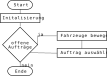
\includegraphics[scale=0.5]{images/greedy-diagram}
    \caption{Ablauf Greedy Ansatz}
    \label{figure:greedy-diagram}
\end{figure}

Im ersten Schritt wird das Fahrtzeug mit der geringsten Distanz zu seinem Ziel gewählt (hat es kein Ziel ist die Distanz \num{0}) und alle Fahrzeuge um diese Distanz bewegt und
geprüft ob ihre jeweiligen Aufträge nun erfüllt sind.

Im nächsten Schritt wird für alle Fahrzeuge welche keinen aktiven Auftrag haben ein nächster
Auftrag ausgewählt. Dieser Schritt unterscheidet sich von dem vorherigen Ansatz,
da hier nun neben der Distanz zwischen Start- und Zielposition des Auftrags auch
das Vorhandensein eines Anschlussauftrags als Parameter für die Heuristik herangezogen wird.
Daher gibt es an der aktuellen Maschine Aufträge, wird der Auftrag ausgewählt, welcher
an seinem Ziel einen Folgeauftrag hat.
Sollte es keine Aufträge an der aktuellen Maschine geben, wird die nächste Maschine angesteuert,
welche noch Aufträge hat.

\subsubsection{Verbesserte Heuristik}
Während der Implementation der Strategie hatte sich gezeigt, dass eine Optimierung der
Heuristik möglich ist, hierfür wurde diese wie folge angepasst:

Statt einfach nur danach zu sortieren ob ein Auftrag einen Folgeauftrag hat,
wird ein Auftrag bewertet nach der Anzahl möglicher Folgeaufträge, daher ein Auftrag
an dessen Ziel mehr Folgeaufträge warten hat eine höhere Priorität.
Sollte es trotzdem noch mehrere Aufträge mit der selben Priorität geben, daher der selben Anzahl
Folgeaufträge, werden diese noch einmal sortiert nach der Distanz des Auftrags,
daher bei gleicher Anzahl Folgeaufträge wird der Auftrag mit der kürzesten Distanz zwischen
Start- und Zielposition gewählt.

Des weiteren im Fall, dass eine Maschine keine Aufträge mehr hat, wird nicht mehr die nächste
Maschine angefahren, sondern die Maschine mit den meisten offenen Aufträgen. Sollte es hier mehrere mit der gleichen Anzahl geben wird hier die Maschine gewählt, zu der aktuell kein
anderes Fahrzeug unterwegs ist.


\subsection{Implementierung}
Der Ansatz wurde mittels \emph{Python} implementiert, die Umsetzung erfolgte größtenteils
mit den mitgelieferten Paketen, einzig das \emph{numpy} Paket wurde zusätzlich verwendet
um die Berechnung der Distanzen zu vereinfachen.

Im ersten Schritt werden die Maschinen erzeugt, diese werden als einfach Tupel ihrer Koordinaten
in einer Liste repräsentiert. Daher der Listenindex entspricht der \emph{ID} der Maschine.
Des weiteren werden die Transportaufträge eingelesen und die Fahrzeuge erstellt, diese werden als Objekte mit den Attributen: ID, Position, Ziel, Distanz zum Ziel und ob sie Ladung transportieren repräsentiert.

Danach werden, in einer \code{WHILE}-Schleife, die Aufträge abgearbeitet.
Dies erfolgt, in dem das Fahrzeug mit der kürzesten Distanz zum Ziel ermittelt wird und
alle Fahrzeuge um diese Distanz bewegt werden und alle aktiven Aufträge auf Erfüllung geprüft werden.
Alle Fahrzeuge, welche nun keinen aktiven Auftrag mehr haben, werden nun mit einem neuen
Auftrag versorgt, dazu werden die oberen Heuristiken verwendet.

Dem Fahrzeug wird ein neues Ziel zugewiesen, sollte eine Fahrt mit Ladung erfolgen,
wird dies im Fahrzeug gespeichert. Des weiteren wird für die spätere Ausgabe der Pfade,
die Fahrt des Fahrzeugs in der Ausgabeliste hinzugefügt.

\subsubsection{Verbesserte Version}
Um die verbesserte Heuristik zu Implementieren wurde die Implementierung der Fahrzeuge,
Aufträge und Maschinen verändert.
Für all diese Objekte wurden Klassen entworfen und Teile der Logik als Klassenmethoden
implementiert, besonders die Implementierung der Fahrzeuge wurde angepasst, sodass jedes
Fahrzeug nun eine Liste an aktuellen Aufträgen enthält, sowie eine Liste aller erledigter Aufträge.

Ein wichtiger Unterschied zur vorhergehenden Version ist das Speichern eines Folgeauftrages
im Falle eines Maschinenwechsels. Daher ein Fahrzeug, welches von einer Maschine, welche keine offenen Aufträge mehr hat, zu einer anderen Maschine unterwegs ist, blockt bereits den dortigen Folgeauftrag.

Somit wird der Fall umgangen, dass ein Fahrzeug zu einer Maschine fährt um dort einen Auftrag
anzunehmen, jedoch ein anderes Fahrzeug schneller war und den Auftrag bereits angenommen hat.
Dies würde sonst zu einer unnötigen Leerfahrt führen.

Erfolgte Fahrten werden nun direkt im Fahrzeug gespeichert, somit werden am Ende für die Ausgabe
die Fahrzeuge durch iteriert und die Liste ihrer Pfade direkt aus der jeweiligen Fahrzeug liste
extrahiert.


\subsection{Ergebnisse}
Aufgrund des Greedy-Ansatzes liefert das Skript die Ergebnisse ohne spürbare Verzögerung,
gemessen wurde eine Ausführungszeit von $\approx \SI{0.205}{\second}$
für die erste Version, respektive $\approx \SI{0.251}{\second}$ für die Verbesserte.

Die Lösungsgüte ist in Tabelle \ref{table:greedy-paths} aufgezeigt.
\begin{table}[H]
    \centering
    \begin{tabularx}{\textwidth}{|*{4}{Y|}}
        \hline
        \multirow{2}{*}{Anzahl Fahrzeuge} & \multicolumn{2}{c|}{Berechneter Wert}\\
                                            \cline{2-3} &Version 1 &Version 2 \\
        \hline
        1    & \num{7757.18}   & \num{7165.10}    \\ \hline
        3    & \num{2612.26}   & \num{2425.26}    \\ \hline
        5    & \num{1577.01}   & \num{1462.75}    \\ \hline
    \end{tabularx}
    \caption{Ergebnisse des Greedy-Ansatzes}
    \label{table:greedy-paths}
\end{table}

\section{Ansatz 3: Ruin and Recreate}
\subsection{Strategie}
Ein weiterer Ansatz zur Berechnung eines möglichst optimalen Ablaufplans ist die Verwendung der \emph{Ruin-and-Recreate}-Strategie beschrieben durch Schrimpf et al. \cite{schrimpf} Dieser Algorithmus verwendet einen iterativen Ansatz, in dem zuerst Teile der Lösung entfernt werden (Ruin-Schritt) und nachfolgend wieder anders zusammengesetzt (Recreate-Schritt) werden. Bei der erneuten Zusammensetzung der Lösung wird dabei ein Ergebnis präferiert, welches eine beschriebene Zielfunktion maximiert - in unserem Anwendungsfall also eine Lösung, die die zurückgelegte Strecke aller Fahrzeuge (und damit die Gesamtausführungszeit des Ablaufplans) minimiert.

\subsection{Implementierung}
Zur Implementation dieser Meta-Heuristik verwenden wir das Java-Framework jSprit, welches auf dem Grundalgorithmus beschrieben durch Schrimpf et al. basiert. Dazu werden unsere bereitgestellten Fahrzeuge durch Objekte der Klasse \code{Vehicle} dargestellt. Diese werden mit einer Gesamtkapazität von 1 erstellt und initial an den korrespondierenden Maschinen positioniert. Die Transportanforderungen aus \emph{transport\_demand.txt} werden in jSprit als Objekte der Klasse \code{Shipment} abgebildet.

Jedes \code{Shipment} hat eine Größe von \emph{1}, es werden also gegebenenfalls mehrere Shipments mit der gleichen Start- und Zielposition erstellt, wenn die Transportanforderungen dies vorgeben. Zusätzlich werden dem Algorithmus noch benutzerdefinierte Constraints vorgegeben, die eine Senkung der maximalen Transportzeit im Recreate-Schritt des Algorithmus bevorzugt. Der Algorithmus wird dann mit einer Obergrenze von \num{2000} Iterationen gestartet.

\subsection{Ergebnisse}
Die Laufzeit des Programms ist direkt abhängig von der Obergrenze der Iterationen,
bei der gesetzten Obergrenze von \num{2000} Iterationen terminiert das Programm
nach $\approx \SI{133.099}{\second}$.
Die Lösungsgüte ist in Tabelle \ref{table:ruin-and-recreate} abgebildet:
%
\begin{table}[H]
    \centering
    \begin{tabular}{|c|c|}
    \hline
    Anzahl Fahrzeuge & Berechneter Wert \\ \hline
    1                & \num{6995.31}    \\ \hline
    3                & \num{2324.02}    \\ \hline
    5                & \num{1389.65}    \\ \hline
    \end{tabular}
    \caption{Ergebnisse ruin-and-recreate}
    \label{table:ruin-and-recreate}
\end{table}

\section{Ergebnisdiskussion}
Der erste und zweite Ansatz basieren jeweils auf einem Greedy-Ansatz, daher es wird bei jeder
Station der zu diesem Moment beste Auftrag ausgewählt.
Dies hat den Vorteil, dass beide Strategien theoretisch dynamisch sich an neue Aufträge anpassen
können, somit könnten während der Fahrt neue Aufträge hinzugefügt oder entfernt werden.
Dies birgt jedoch auch den Nachteil, dass diese Strategien keine optimale Lösung bieten.

Im Vergleich dazu zeigt die dritte Strategie eine deutlich bessere Lösungsgüte,
jedoch wieder mit dem Nachteil, das eine vorherige Berechnung stattfinden muss und eine
Veränderung der Aufträge eine neue Berechnung zur Folge hätte.

Somit hängt es vom Anwendungsfall ab, ob eine Berechnung im Voraus möglich ist oder
ob ein Kompromiss bei der Lösungsgüte möglich ist.
Vergleicht man die Ergebnisse so erkannt man in der Gegenüberstellung \ref{table:compare-strategies},
dass der erste Greedy-Ansatz kaum eine Verbesserung gegenüber dem Kürzeste-Distanz Ansatz bringt.
Jedoch die verbesserte Version beiden deutlich überlegen ist.
Der \emph{Ruin-and-Recreate}-Ansatz ist noch um $\approx \SI{3.85}{\percent}$ besser als der
zweite Greedy-Ansatz, jedoch auf Kosten einer um $\approx \SI{530}{\percent}$ höheren Laufzeit.

\begin{table}[H]
    \centering
    \begin{tabular}{|c|r|r|r|}
    \hline\centering
    Strategie & \multicolumn{1}{c|}{1} & \multicolumn{1}{c|}{2.1} & \multicolumn{1}{c|}{2.2}
                                                                                        \\ \hline
    1         & 0                      & -                        & -                   \\ \hline
    2.1       & \SI{ 1.83}{\percent}   & 0                        & -                   \\ \hline
    2.2       & \SI{ 9.04}{\percent}   & \SI{ 7.35}{\percent}     & 0                   \\ \hline
    3         & \SI{12.53}{\percent}   & \SI{10.91}{\percent}     & \SI{3.85}{\percent} \\ \hline
    \end{tabular}
    \caption{Verbesserung der Ergebnisse, gemittelt aus den Verbesserungen der jeweiligen Ergebnissen (ein, drei und fünf Fahrzeuge).}
    \label{table:compare-strategies}
\end{table}

\chapter{Aufgabe 2}
\section{Initiale Probleme}
Bei der Umsetzung von Aufgabe 2 wurde zur Programmierung von der hauseigenen Lego Software abgesehen. Leider wollte uns die Benutzung des \code{repeat until}-Blockes, welcher eine while-Schleife abbilden soll, nicht gelingen. Sowohl die Bedingung $x < y$ als auch $x > y$ führten nicht zum gewünschten Verhalten. Nur bei $x = y$ zeigte der Roboter eine Reaktion.

Da das Programm die Rotation der Motoren allerdings in zu großen Abständen abtastet, wurde nie exakt die 2-Meter-Marke gemessen und somit überfahren. Aufgrund dessen wurde nach einer Alternative gesucht. Der Hinweis der Tutoren, die alte Softwareversion zu benutzen, kam leider zu spät.

Das \emph{MicroPython\,Package}, welches ebenfalls von Lego bereitgestellt wird, bot sich hierfür bestens an. Außerdem ermöglichte das eine einfachere Einarbeitung durch Python-Vorkenntnisse, verständlicheren Code und Kollaboration durch Verwendung von Git.


\section{Experiment 1: Freie Fahrt}
\subsection{Aufgabenstellung}
Das Fahrzeug soll ohne weitere Sensorik eine Strecke von $\SI{2}{\m}$ geradeaus zurücklegen.

\subsection{Herangehensweise}
Die Geschwindigkeit des Motors setzen wir initial auf $440$, da dies scheinbar die Maximalgeschwindigkeit ist. Um die zurückgelegte Strecke des Roboters zu ermitteln, muss die Rotation des Motors gemessen werden. Mit Hilfe der Funktion \code{motor.angle()} wird die Motorstellung in Grad ausgelesen und kann mit Hilfe des Radumfangs $d$ in eine Strecke umgerechnet werden.
%
\begin{equation}
    \label{equation:2meterstrecke}
    \begin{aligned}
       d &= \SI{56}{\mm}\\
       u &= \pi \cdot d \approx \SI{176}{\mm} \\
       y &= \frac{\SI{2}{\m}}{u} \cdot \SI{360}{\degree} \approx \SI{4092.6}{\degree}
    \end{aligned}
 \end{equation}
 %
Nach Gleichung \ref{equation:2meterstrecke} entsprechen 2 Meter also ca. \SI{4092.6}{\degree}.

\subsection{Herausforderungen bei der Problemstellung}
Leider mussten wir feststellen, dass der errechnete Werte stark von der Realität abweicht. Nach einem Testlauf haben wir den Wert manuell auf $y = \SI{3870}{\degree}$ eingestellt. Wir ließen den Roboter mehrmals die Strecke abfahren und ermittelten dabei die benötigte Zeit per Stoppuhr und die Abweichung von der erwarteten Zielposition. Letzteres unterteilten wir in zwei Messreihen: Abweichung in der Länge, also ob der Roboter zu kurz oder übers Ziel hinaus gefahren ist. Und Abweichung in der Breite, also ob der Roboter nach links oder rechts lenkt.

\subsection{Auswertung}
Es gibt verschiedene Gründe für die Abweichung zwischen dem berechneten und gemessenen Gradmaß. Dazu zählen Messfehler sowohl beim Aufbau der Testumgebung als auch bei der Ermittlung des Raddurchmessers. Durch das Gewicht des Roboters kann außerdem der Reifen zusammengedrückt werden, was zu einer Veränderung des Raddurchmessers führt. Weiterhin erfolgt das Bremsen des Roboters nicht durch aktives Abbremsen, sondern durch Ausrollen der Motoren. Dadurch schaltet der Roboter bei Erreichen der gewünschten Radrotation $y$ zwar die Motoren ab, kommt jedoch erst ein paar Zentimeter später zum Stehen. Letztlich können auch Fehler bei der Startaufstellung des Roboters, wie beispielsweise Über- oder Unterschreiten der Startlinie und der initialen Stellung des Hinterrads auftreten.

Tabelle \ref{table:zeitmessung} zeigt die Ergebnisse der Zeitmessung. Die Streuung der Messergebnisse ist sehr klein und ist wahrscheinlich stark von Messfehlern beeinträchtigt, sodass wir 10 Zeitmessungen als ausreichend empfanden und wir uns keine neuen Erkenntnisse von weiteren Messungen erhofften.
%
\begin{table}[H]
    \centering
    \begin{tabular}{|c|c|}
    \hline
    Mean               & $\SI{5,65}{\s}$ \\ \hline
    Standardabweichung & $\SI{0,09}{\s}$ \\ \hline
    Min                & $\SI{5,47}{\s}$ \\ \hline
    Max                & $\SI{5,78}{\s}$ \\ \hline
    \end{tabular}
    \caption{Zeitmessung}
    \label{table:zeitmessung}
\end{table}
%
Tabelle \ref{table:laengenabweichung} stellt die Abweichung von der erwarteten Zielposition in der Länge dar. Ein optimales Ergebnis wird hier mit $\SI{0}{\mm}$ repräsentiert, während negative Werte für zu kurze Fahrten und positive Werte für zu lange Fahrten stehen. Den stärksten Fehlereinfluss auf die Streuung hier hat wahrscheinlich die Variation der initiale Startposition des Roboters.
%
\begin{table}[H]
    \centering
    \begin{tabular}{|c|c|}
    \hline
    Mean               & $\SI{-10,18}{\mm}$ \\ \hline
    Standardabweichung & $\SI{3,24}{\mm}$ \\ \hline
    Min                & $\SI{-19}{\mm}$ \\ \hline
    Max                & $\SI{-3}{\mm}$ \\ \hline
    \end{tabular}
    \caption{Längenabweichung}
    \label{table:laengenabweichung}
\end{table}
%
Die Verteilung der Daten, wie im Histogramm in Abbildung \ref{figure:laengenverteilung} zu sehen, lässt auf eine annähernde Normalverteilung der Messwerte schließen. Diese Erkenntnis kann genutzt werden, um den Roboter erneut zu kalibrieren. Diese kleine Abweichung konnte bei der initialen Kalibrierung nur schwer bemerkt werden, summiert sich allerdings bei hoher Anzahl an Fahrten auf uns sorgt für Probleme und Ineffizienzen.
%
\begin{figure}[H]
    \centering
    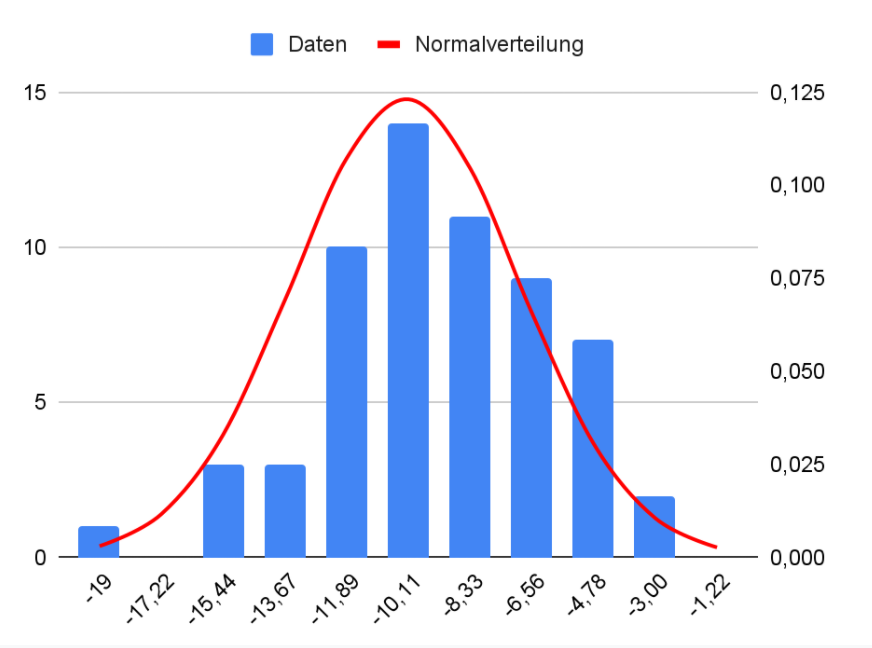
\includegraphics[scale=0.5]{images/laengenverteilung.png}
    \caption{Längenverteilung}
    \label{figure:laengenverteilung}
\end{figure}
%
Tabelle \ref{table:breitenabweichung} stellt die Abweichung von der erwarteten Zielposition in der Breite dar. Ein optimales Ergebnis wird wieder mit $\SI{0}{\mm}$ repräsentiert, während negative Werte für eine Linkslenkung und positive Werte für eine Rechtslenkung stehen.
%
\begin{table}[H]
    \centering
    \begin{tabular}{|c|c|}
    \hline
    Mean               & $\SI{-35,98}{\mm}$ \\ \hline
    Standardabweichung & $\SI{31,15}{\mm}$ \\ \hline
    Min                & $\SI{-121}{\mm}$ \\ \hline
    Max                & $\SI{25}{\mm}$ \\ \hline
    \end{tabular}
    \caption{Breitenabweichung}
    \label{table:breitenabweichung}
\end{table}
%
Es liegen höchstwahrscheinlich die selben Gründe für Abweichung vor. Allerdings ist eine stärkere Streuung zu erkennen. Begründet werden kann dies mit dem Verhältnis von Längen- und Breitenabweichung. Mathematisch gesehen führt eine Abweichung von $\SI{100}{\mm}$ zu einer Fahrtstrecke von $\SI{2002,5}{\mm}$, bevor der Roboter die Ziellinie überquert. Dabei wird eine gerade Strecke angenommen. Sollte einer der Motoren weniger Leistung als der andere liefern, führt das zu einer Kurvenfahrt. Dies könnte man überprüfen, indem man Messwerte auf halber Strecke oder noch öfter ermittelt. Da der Roboter per Programmierung nur 2 Meter zurückgelegt, führt das zu einer Längenabweichung von $\SI{2,5}{\mm}$. Der Verhältnis von Längen- zu Breitenabweichung beträgt also $1:40$.

Auch im Histogramm in Abbildung \ref{figure:breitenverteilung} lässt sich eine Normalverteilung der Messwerte erkennen. Wie auch bei der Längenabweichung kann diese Erkenntnis zur nachträglichen Kalibrierung genutzt werden. Da man aber annehmen kann, dass sich die Startposition über viele Versuche hinweg mittelt, wird klar, dass der Roboter womöglich einen leichten Linksdrall hat. Auch das kann bei der Kalibrierung berücksichtigt werden. Möglicherweise liegt aber auch ein technischer Defekt oder Verschleiß vor. Des Weiteren besteht trotz Kalibrierung eine große Streuung. Dies kann ausschließlich gelöst werden, indem der Roboter sich per Sensorik an der Linie orientiert. 
%
\begin{figure}[H]
    \centering
    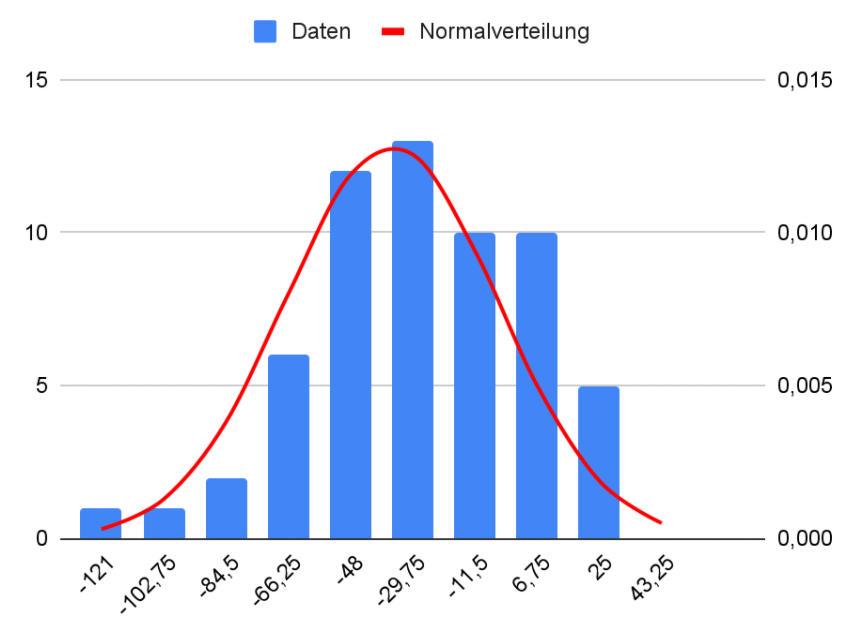
\includegraphics[scale=0.5]{images/breitenverteilung.png}
    \caption{Längenverteilung}
    \label{figure:breitenverteilung}
\end{figure}

\section{Experiment 2: Folgen einer Spur}
\subsection{Aufgabenstellung}
Das Fahrzeug soll mit seiner Sensorik eine Strecke von $\SI{2}{\m}$ geradeaus zurücklegen.

\subsection{Herangehensweise}
Für diese Aufgabe muss der Farbsensor des Roboters einbezogen werden. Um die Messwerte des Sensors in die Programmierung des Roboters mit einzubeziehen, wurde ein Proportional-Controller genutzt. Ein PID-Controller würde vermutlich für kaum merkbare Verbesserung sorgen, steigert die Komplexität allerdings extrem. Damit der Farbsensor möglichst aussagekräftige und unterscheidbare Werte liefert, nutzen wir weißes Tape auf einem schwarzen Tisch, was für starke Kontraste sorgt.

\subsection{Herausforderungen bei der Problemlösung}
Die größte Schwierigkeit bei dieser Aufgabe besteht in der Kalibrierung des P-Controllers. Allerdings lässt sich bei nur einer Regelgröße relativ schnell ein geeigneter Parameter finden. Ein weiteres Problem stellt der Lichteinfall dar. Durch Sonneneinstrahlung oder Lampenreflektion könnten die Sensormesswerte verfälscht werden. Am besten lässt sich das Experiment vermutlich im Dunkeln durchführen, da der Sensor sein eigenes Licht mitbringt. Bereits genannte Gründe für Abweichung kommen auch hier wieder zum tragen, wobei der Roboter Ungenauigkeiten in der Startposition relativ schnell kompensieren kann.

\subsection{Auswertung}
Tabelle \ref{table:zeitmessung2} zeigt die Ergebnisse der Zeitmessung. Auch hier ist die Streuung sehr klein und wahrscheinlich stark von Messfehlern abhängig. Jedoch lässt sich eine minimale Verbesserung zu den Werten des ersten Experiments feststellen. Dies würde sich mit einer geringeren Abweichung von der erwarteten Zielposition erklären lassen.
%
\begin{table}[H]
    \centering
    \begin{tabular}{|c|c|}
    \hline
    Mean               & $\SI{5,65}{\mm}$ \\ \hline
    Standardabweichung & $\SI{0,08}{\mm}$ \\ \hline
    Min                & $\SI{5,52}{\mm}$ \\ \hline
    Max                & $\SI{5,78}{\mm}$ \\ \hline
    \end{tabular}
    \caption{Zeitmessung}
    \label{table:zeitmessung2}
\end{table}

\section{Experiment 3: Umfahren eines Hindernisses}
\subsection{Aufgabenstellung}
Das Fahrzeug soll mit Hilfe seiner Sensorik eine definierte Strecke abfahren und dabei ein fiktives Hindernis umfahren.

\subsection{Herangehensweise}
Theoretisch besitzt der Roboter bereits alle nötigen Fähigkeiten, um auch einer abbiegenden Linie zu folgen. Allerdings wird ihn die Geschwindigkeit aus der Bahn werfen. Zu testen wäre also die größtmögliche Geschwindigkeit, bei der der Kurs verlässlich abgefahren werden kann. Diese Geschwindigkeit kann dann mit dem Erweitern des P-Controller zu einem PID-Controller verbessert werden.

\subsection{Herausforderungen bei der Problemlösung}
Die richtigen Parameter für einen PID-Controller zu finden stellt sich als äußerst komplex dar. Scheinbar gibt es dabei auch keine Best-Practices sondern man muss einfach probieren. \enquote{Verlässliche} Einstellungen des Roboters definieren wird so, dass er den Kurs zehn mal in Folge erfolgreich absolvieren muss.

\subsection{Auswertung}
Für die Testläufe mit dem P-Controller erreichten wir eine maximale Geschwindigkeit von $100$. Diese konnten wir mit dem PID-Controller auf $140$ verbessern. Der Roboter absolvierte auch einzelne Testläufe mit höheren Geschwindigkeiten erfolgreich, jedoch nicht zuverlässig.

Tabelle \ref{table:zeitmessung3} enthält die Ergebnisse der Zeitmessung, auch hier liegen die Messergebnisse wieder stark beieinander. Allerdings unterscheiden sie sich, wie erwartet, stark von den vorherigen Experimenten. Mean und Standardabweichung haben sich in etwa verdoppelt.
%
\begin{table}[H]
    \centering
    \begin{tabular}{|c|c|}
    \hline
    Mean               & $\SI{13,53}{\mm}$ \\ \hline
    Standardabweichung & $\SI{0,13}{\mm}$ \\ \hline
    Min                & $\SI{13,26}{\mm}$ \\ \hline
    Max                & $\SI{13,71}{\mm}$ \\ \hline
    \end{tabular}
    \caption{Zeitmessung}
    \label{table:zeitmessung3}
\end{table}
%
Weitere Optimierung sind möglich, indem man die Parameter des PID-Controllers verbessert. Jedoch ist nicht klar, wann ein Optimum erreicht ist und kann somit unendlich viel Zeit kosten. Des Weiteren hätte der Roboter einen Vorteil, wenn die Abbiegungen der Strecke eher Kurven wären oder zumindest einen stumpferen Winkel hätten. Leider kann der Roboter in diesem Versuchsaufbau keinen Nutzen aus seinem Ultraschallsensor ziehen. Sollte er auf ein Hindernis zufahren, würde er dies frühzeitig erkennen, seine Geschwindigkeit reduzieren, die Kurve sauber fahren und danach wieder beschleunigen. Falls in einem realen Szenario kein Hindernis im Weg sein sollte, sondern ausschließlich Einschränkungen der Route, könnte man dies dem Roboter über eine Karte, Matrix oder einen Graphen mitteilen, sodass er ebenfalls im Voraus auf Kurven reagieren kann.

\chapter{Aufgabe 3}
In der Aufgabenstellung werden Annahmen getroffen, welches das gesamte Konzept simplifizieren. Im Folgenden wollen wir betrachten, welche möglichen Auswirkungen die Realität auf das gegebene Szenario hat, wenn also diese Annahmen nicht mehr gemacht werden können.

\section{Platzbedarf}
\begin{displayquote}
    ``Es befinden sich keine statischen oder dynamischen Hindernisse im Layout. [...] Die gesamte Fläche ist befahrbar. [...] Alle Fahrzeuge fahren auf direktem Weg zwischen den Maschinen (euklidische Distanz).'' \cite{aufgabenstellung}
\end{displayquote}
%
Ein Unternehmen, welches autonome Transportsysteme so effizient wie möglich einsetzen möchte, wird sicherlich auch den zur Verfügung stehenden Platz in ihrer Logistikhalle sinnvoll nutzen wollen. Flächen frei zu lassen, nur damit die Fahrzeug nicht mit Hindernissen kollidieren können, stellt sich in den meisten Fällen wahrscheinlich aus unökonomisch heraus. Dynamische Hindernisse im Sinne anderer Roboter kann vergleichsweise einfach gelöst werden, indem die Fahrzeuge die Positionen der anderen Fahrzeuge übermittelt bekommen und dementsprechend reagieren können. Menschen als dynamische Hindernisse stellen sich womöglich als größeres Problem dar. Moderne Kamerasysteme können evtl. visuell ihre Umgebung wahrnehmen, Personen erkennen und bremsen bzw. ausweichen, jedoch ist das mit großen Kosten für Technik verbunden und das System muss einwandfrei funktionieren um Arbeitsunfälle zu vermeiden. Sollten Kamerasysteme solcher Art nicht zum Einsatz kommen, gebietet der Arbeitsschutz eine klare, mindestens visuelle, Abtrennung des Bereiches für die Fahrzeuge und des begehbaren Bereiches für Personen. Die kollidiert allerdings wiederum mit der Annahme, die gesamte Fläche sei befahrbar. Eine Mögliche Lösung wäre, das Transportsystem auf eine tiefer oder höher liegende Ebene zu verlegen. Somit wäre zumindest die Fahrzeug- und Personendomäne getrennt.

\section{Auftragszeit und -reihenfolge}
\begin{displayquote}
    ``Ein einzelner Auftrag hat keinen bestimmten Liefer- oder Abholzeitpunkt. [...] Die Aufträge sind homogen, d.h. es liegen keine geforderte Reihenfolge oder Priorisierung vor.'' \cite{aufgabenstellung}
\end{displayquote}
%
Bei Unternehmen, in denen 24/7 gearbeitet wird, muss der Auftragspool entweder nach einer gewissen Zeit abgearbeitet sein und dann neu gestartet werden, was mit Overhead und damit Ineffizienz verbunden ist. Oder die zu transportierenden Güter bekommen ein weiteres Deadline-Attribut, welches im Scheduling-Algorithmus mit einbezogen werden muss. Unternehmen, bei denen das nicht der Fall ist, könnten ihren Zeithorizont der Arbeitszeit anpassen. Das bedeutet, am Ende des Tages ist der Aufgabenpool abgearbeitet. Allerdings können das zwischendrin keine neuen Aufträge eingepflegt werden und man kann nicht erwarten, dass bestimmt Aufträge eher fertig werden als andere. Dafür müssten diese Unternehmen dann ebenfalls den Auftragspool neu starten oder Prioritäten vergeben.

\section{Treibstoff und Verschleiß}
\begin{displayquote}
    ``Fahrzeuge sind zu 100\% einsatzbereit und fallen nie aus. [...] Fahrzeuge haben eine unendliche Reichweite, können also unendlich weit/lange fahren.'' \cite{aufgabenstellung}
\end{displayquote}
%
Da Verschleiß und Energievorrat immer eine Rollen spielen, kommt es in der Realität unvermeidlich zu Ausfällen. Selbst bei unseren Experimenten in Aufgabe 2 ist während der Durchführung der Roboter wegen zu niedrigem Akkustand ausgefallen. Man kann dies natürlich mit zusätzlicher Sensorik überwachen um rechtzeitig den Roboter zu warten. Allerdings bedeutet das an sich schon einen Ausfall für den Roboter und ist zusätzlich mit Hardware- und Personalkosten verbunden.

\section{Be- und Entladezeiten}
\begin{displayquote}
    ``Es fallen keine Tot-, Neben- und Handhabungszeiten an.'' \cite{aufgabenstellung}
\end{displayquote}
%
Natürlich ist in der Realität das Be- und Entladen mit einem gewissen Zeitaufwand verbunden. Diesen kann man allerdings minimal und über verschiedene Maschinen hinweg gleich halten, wenn ein effizientes Be- und Entladungssystem zum Einsatz kommt.

\section{Fahrzeugkollisionen}
\begin{displayquote}
    ``Die Fahrzeuge sind dimensionslos, d.h. Es finden keine Konflikte zwischen den Fahrzeugen statt, womit keine Ausweichmanöver von Nöten sind.'' \cite{aufgabenstellung}
\end{displayquote}
%
Wie die bereitgestellten Videos der Simulation gezeigt haben, ist diese Annahme weit von der Realität entfernt. Es wurden dabei ausschließlich Beschleunigung und Dimension der Roboter einbezogen, was bereits zu einer \SIrange{16}{65}{\percent} längeren Bearbeitungszeit führt. Bei der Kollisionsdetektion und des Ausweichmanövern gibt es eventuell noch etwas Verbesserungspotential. Des Weiteren könnte man einen Parameter hinzufügen, welcher die Anzahl an Kollisionen zählt und vom Algorithmus minimiert werden sollte. Jedoch führt eine minimal Kollisionszahl wahrscheinlich nicht immer zu besseren Zeiten, da die Roboter dann Umwege fahren müssten.

\section{Maschinenkollisionen}
\begin{displayquote}
    ``Die Maschinen sind dimensionslos, d.h. die Fahrzeuge fahren exakt zu den angegebenen Koordinaten der Maschinen, um ein Transportgut aufzunehmen oder abzugeben.'' \cite{aufgabenstellung}
\end{displayquote}
%
Mit hoher Wahrscheinlichkeit muss der Roboter in der Realität auch mal die ein oder andere Maschine umfahren. Wie die Erkenntnisse aus Aufgabe 2 zeigen, benötigt der Roboter beim Umfahren von Hindernissen im Vergleich zu einer geraden Strecke mindestens das 2,5fache der Zeit. Allerdings spielt die Dimension der Maschinen bei dem gegebenen Hallenlayout, und auch bei ähnlichen Layouts, eine relativ geringe Rolle. Die Koordinaten sind mehr oder weniger kreisförmig angeordnet, sodass eine Kollision mit einer Maschine womöglich vermieden werden kann, wenn sich die Roboter nur im Kreisinneren aufhalten. Allerdings führt, wie bereits beschrieben, ein möglichst freier Raum auf den Routen der Roboter zu großem Platzbedarf und somit erhöhten Kosten und Ineffizienzen.

\section{Beschleunigung}
\begin{displayquote}
    ``Fahrzeuge fahren durchgängig mit der maximalen Geschwindigkeit von 1 Streckeneinheit/Zeit.'' \cite{aufgabenstellung}
\end{displayquote}
%
Aus hier gibt die Simulation Aufschluss über das Verhalten in der Realität. Wie viel des zusätzlichen Zeitbedarfs jeweils der Beschleunigung oder dem Kollidieren der Roboter zuzuschreiben ist, lässt sich schwer sagen. Fakt ist jedoch, das positive und negative Beschleunigung Zeit kosten. Mit stärkere Motorisierung und besseren Bremsen könnte dies verbessert werden, doch auch hier spielt die Kostenabwägung einer entscheidende Rolle. Ebenso zeigen die Ergebnisse der Experimente, dass ein Abbremsen vor dem Umfahren eines Hindernisses zu besseren Resultaten führt. Das würde natürlich die Anzahl an Beschleunigungsmanövern erneut erhöhen und müsste mit der Gesamtzeitersparnis ins Verhältnis gesetzt werden.

\section{Größe der Fahrzeugflotte}
Die Ergebnisse in Aufgabe 1 deuten auf eine lineare Abnahme der Zeit mit steigender Roboteranzahl hin. Ein Fahrzeug pro Auftrag wäre also mit den getroffenen Annahmen die optimale Lösung. Jedoch werden viele der bereits genannten Probleme mit steigender Anzahl von Fahrzeugen verstärkt, sodass ab einer bestimmten Zahl die benötigte Zeit nicht mehr abnimmt und unter Umständen sogar steigt. Auch die Erhöhung der Maschinenanzahl kann hier nur bedingt Abhilfe schaffen, da sich dennoch viele Routen der Roboter kreuzen und die Kollisionsanzahl hoch bleibt.

\bibliographystyle{unsrt}
\bibliography{bibliography}

\end{document}
